\subsection{Audio-based trigger module}
As described in study section, we decided to use Support Vector Machine (SVM) as underlying machine learning algorithm and Mel-Frequency Cepstral Coefficients (MFCC) as feature set for this algorithm  to detect scream. Let's have a look at feature extraction procedure used in this project.
\subsubsection{Feature Extraction}
Mel-Frequency Cepstral Coefficients (MFCC), which acts as feature set, are extracted from live stream of input audio. Figure~\ref{fig:Featureextraction} depicts the Feature extraction procedure.

\begin{figure}[H]
\centering
\def\svgwidth{\textwidth}
\input{feat.pdf_tex}
\caption{Feature extraction process}
\label{fig:Featureextraction}
\end{figure}

Every second audio data is fetched from sound card and dumped into an input fifo, this 1 second of audio data is then appended with previous 0.98 second (0.98 second is multiple of 30 ms, which is the window size used in the FFT operation) of audio data. MFCC features are extracted for this composite audio clip.

MFCC are computed by first chopping the audio signal into tiny overlapping segments, these segments are multiplied with a window function like Hamming window; Fourier transform is computed over this windowed audio segment. The power spectrum is wrapped according to Mel-scale to adapt the frequency resolution of human ear. This spectrum is then segmented into number of critical bands using a triangular filter bank; Inverse Discrete Cosine Transform (DCT) applied to the logarithm of filter bank's outputs result in MFCC vector.

We obtain super feature vector of R\textsuperscript{24} for each 1.98 sec of audio data. This super feature vector is obtained by taking column mean and standard deviation of 169 x 12 matrix, which was obtained by extracting MFCC(ignoring 0\textsuperscript{th} MFC coefficient) for audio data of 1.98 sec. Once features are extracted, they are used for training the SVM.  

\subsubsection{Training of SVM}
\paragraph{Training-\\}

Like all machine learning algorithms, we need to train our SVM using a labeled data set. Labeled data set contains data that is painstakingly labeled by a human, classifying whether a particular 1.98 second clip is a scream. Clip is labeled 1 for a scream and -1 for not a scream. Figure~\ref{fig:train} depicts the training process.
 
\begin{figure}[H]
\centering
\def\svgwidth{\textwidth}
\input{train.pdf_tex}
\caption{Training process of the SVM}
\label{fig:train}
\end{figure} 
Support Vector Machine (SVM) uses a kernel to transform data into higher dimension space and finds a linear separating hyper plane with maximal margin in this higher dimensional space. We are using radial basis function (RBF) as kernel, due to its ability to model complex data patterns. RBF kernel \(K(x_i,x_j)\)
is defined as- \[K(x_i,x_j)=exp(-\gamma\parallel(x_i-x_j)\parallel^2), \gamma>0.\]
For training SVM that uses RBF kernel, we need to specify values of two parameters -
\begin{enumerate}
 \item C (penalty factor used in cost function) and 
 \item \(\gamma\) ( variance of the RBF kernel).
\end{enumerate}
 We used following steps to get optimum value of C and \(\gamma\) and use them for the training-
\begin{enumerate}
\item Arrange data in proper format i.e., [data,label],
\item Randomize the data in cross-validation set,
\item Consider the RBF kernel \(K(x,y)=e^{(-\gamma\parallel(x_i-x_j)\parallel^2)}\),
\item Use cross-validation set to find the best values for parameters C and \(\gamma\),
\item Use these values of C and \(\gamma\), to train the SVM from training data set and
\item test.
\end{enumerate}

We will dwell into details of these steps in section \ref{sssec:FindCandgamma}, first lets have a look at data set used in this project. 

\paragraph{Data set-\\}

Data set used in this project is called IIITD Urban Environment Context database (IUEC)\cite{paper10}. It contains audio clips from following environmental contexts-
\begin{enumerate}
\item Conversation (narrations)
\item Human gathering (clubs and meetings)
\item Indoors (indoor sounds)
\item machinery (fan, shaver, laptop-fan, exhaust, oven, mixer, washing machine and vacuum cleaner)
\item Multimedia (movie audio and TV audio)
\item Outdoors (bus stand, road traffic, market, temple, rickshaw, rain, metro and playground)
\item distress (scream and crying sounds)
\end{enumerate}

Table~\ref{tab:quandata} quantifies the content of this dataset.
\begin{table}[H]
\begin{center}
\begin{tabular}{ |c|c| } 
 \hline
 \textbf{Context} & \textbf{Samples of 2 sec} \\ 
 \hline
 \hline
 Conversation & 623 \\
 \hline 
 Human gathering & 1621 \\ 
 \hline
 Indoors & 4169 \\
 \hline
 Machinery & 3548 \\
 \hline
 Multimedia & 3698 \\
 \hline
 Outdoors & 5142 \\
 \hline
 Scream & 464 \\
 \hline
 \hline
 \textbf{Total} & \textbf{19265= 10 Hrs 42 Mins}\\
 \hline
\end{tabular}
\end{center}
\caption{IUEC Data set details} \label{tab:quandata}
\end{table}

Apart from this data set, we collected data using the \emph{PanicButton device} prototype. Table~\ref{tab:quandata2} quantifies its content.
\begin{table}[H]
\begin{center}
\begin{tabular}{ |c|c| } 
 \hline
 \textbf{Context} & \textbf{Samples of 2 sec} \\ 
 \hline
 \hline
 Conversation & 1144 \\ 
 \hline
 Multimedia & 1828 \\
 \hline
 Outdoors & 2623 \\
 \hline
 Scream & 464 \\
 \hline
 \hline
 \textbf{Total} & \textbf{6059= 3 Hrs 22 Mins}\\
 \hline
\end{tabular}
\end{center}
\caption{Details of data collected from panic button prototype} \label{tab:quandata2}
\end{table}

Scream samples were obtained by re-recording scream data available in IUEC data set. We combined this two data sets to get a composite data set, whose content is quantified in Table~\ref{tab:quandata3}
\begin{table}[H]
\begin{center}
\begin{tabular}{ |c|c| } 
 \hline
 \textbf{Context} & \textbf{Samples of 2 sec} \\ 
 \hline
 \hline
 Conversation & 1767 \\
 \hline 
 Human gathering & 1621 \\ 
 \hline
 Indoors & 4169 \\
 \hline
 Machinery & 3548 \\
 \hline
 Multimedia & 5526 \\
 \hline
 Outdoors & 7765 \\
 \hline
 Scream & 928 (3.6\% of complete data set)\\
 \hline
 \hline
 \textbf{Total} & \textbf{25324= 14 Hrs 4 Mins}\\
 \hline
\end{tabular}
\end{center}
\caption{Composite Data set details} \label{tab:quandata3}
\end{table}

This complete data set gets divided into two equal parts called training data set and cross-validation data set. Training data set is used for training the SVM and cross-validation dataset is used for tuning the SVM. Our data set is highly skewed i.e., scream samples constitutes only 3.6\% of the complete data set. This makes benchmarking of trained SVMs non-conventional. Section~\ref{sssec:FindCandgamma} addresses this problem in detail.

Finally, a test clip of 22 minutes was created to quantify performance of the trained SVM. This 22 minute clip was carefully designed to cover audio samples from every context. Obtained results are mentioned in Section~\ref{sssec:performanceSVM}.

\subsubsection{Finding C and gamma} 
\label{sssec:FindCandgamma}
To find the optimum value of C and \(\gamma\), we performed grid search for these parameters on cross-validation data set. Five fold cross-validation data set (4 part for training and 1 part for testing in circular fashion for a particular combination of C and \(\gamma\)) is used. Figure~\ref{fig:CVflowchart} shows the process of finding optimum C and \(\gamma\).

\begin{figure}[H]
\centering
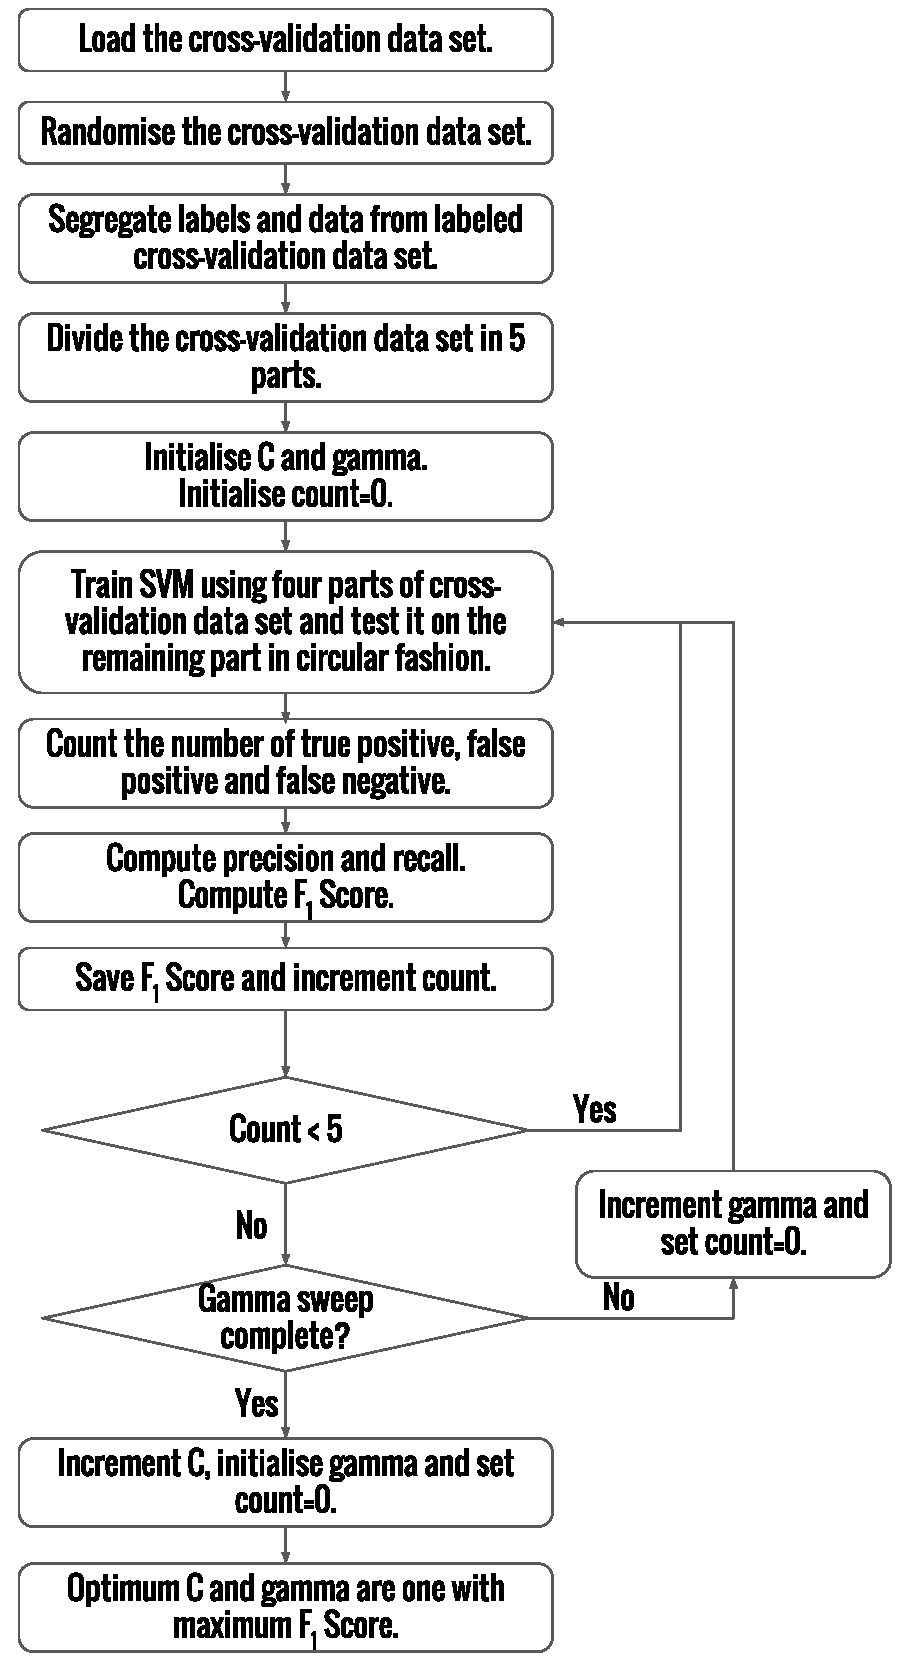
\includegraphics[scale=0.85]{CVflowchart.pdf}
\caption{Cross-validation process for obtaining optimum C and gamma}
\label{fig:CVflowchart}
\end{figure}

Method shown in figure~\ref{fig:CVflowchart} is a brute force method to find optimum value of C and \(\gamma\). We use \(F_1\) score as figure of merit (FOM); Accuracy can't be used as FOM due to skewed nature of data set.

\(F_1\) score is computed using precision (prec) and recall (rec):\[F_1=\dfrac{2 . prec . rec}{prec+rec},\] We can compute precision and recall by: \[prec=\dfrac{t_p}{t_p+f_p}\]
\[rec=\dfrac{t_p}{t_p+f_n}\]
where
\begin{itemize}
\item \(t_p\) is the number of true positives: the ground truth label says it's a scream and our algorithm correctly classified it as a scream.
\item \(f_p\) is the number of false positives: the ground truth label says it's \textbf{not} a scream, but our algorithm incorrectly classified it as a scream.
\item \(f_n\) is the number of false negatives: the ground truth label says it's a scream, but our algorithm incorrectly classified it as \textbf{not} a scream.
\end{itemize}

In any automated alarm system, ideally we should have zero false negative, practically it should be as small as possible. Following figure show us the $F_1$ score obtained by performing grid search for the parameters C and \(\gamma\) on the cross-validation set.
\begin{figure}[H]
\centering
\def\svgwidth{\textwidth}
\input{F1score.pdf_tex}
\caption{F1 score obtained from grid search for C and gamma on CV set}
\label{fig:f1score}
\end{figure} 

Once we have the value of C and \(\gamma\), we can use that value to train our SVM. This process of first obtaining appropriate value of C and \(\gamma\) and then training the final SVM, helps us in avoiding machine learning traps like over-fitting and under-fitting.
Performance of the trained SVM is quantified in section~\ref{sssec:performanceSVM}, besides figure~\ref{fig:f1score} also quantifies the performance of best SVM, over the five fold cross-validation set.

\subsubsection{Performance of the SVM}
\label{sssec:performanceSVM}

We performed benchmarking using a 22 minute test set, this test set contains 24 screams of different lengths and strengths. We were able to detect 23 screams with 1 false negative and 3 false positive, giving us accuracy of \textbf{95.8\%} and \(F_1\) score of \textbf{0.92} with latency of 1.480 ms.

